%! Author = Stepan Oskin
%! Date = 11-Jul-19

% Preamble
\documentclass[11pt]{article}

% Packages
\usepackage{amsmath, subcaption}
\usepackage{graphicx}

% New commands
\newcommand{\norm}[1]{\left\lVert#1\right\rVert}
\newcommand{\vect}[1]{\boldsymbol{#1}}
\newcommand{\pa}[1]{\partial{#1}}

% Document
\begin{document}

    \title{Mathematics of the Logistic Regression \\
    Excerpts from Python Machine Learning \\
    Second Edition \\
    By Sebastian Raschka and Vahid Mirjalili\cite{RaschkaMirjalili2017} \\
    and other sources}

    \author{Stepan Oskin}

    \maketitle

    \begin{abstract}


    \end{abstract}

    \section{Introduction} \label{sec:ada_intro}

    \subsection{Classification} \label{subsec:classification}

    Classifying data is a common task in machine learning.
    Suppose some given data points each belong to one of two classes, and the goal is to decide which class a
    new data point will be in.

    In the case of the Logistic Regression learning algorithm, a data point is viewed as a $p$-dimensional vector
    (a list of $p$ numbers), and we want to know whether we can separate such points with a $(p-1)$-dimensional hyperplane.
    This is called a linear classifier.
    More formally, we can put the idea behind artificial neurons into the context of a binary classification task where we refer to our two classes as 1 (positive class) and -1 (negative class) for simplicity.
    There are many hyperplanes that might classify the data.
    We can then define a decision function ($\phi(z)$) that takes a linear combination of certain input values $x$ and a corresponding weight vector $w$, where $z$ is the so-called net input.
    Models for binary classification can be extended to multi-class classification, for example, via the One-versus-Rest (OvR) technique.

    \subsection{Perceptron vs Logistic Regression} \label{subsec:lr_intro}

    Similar to the perceptron\cite{Rosenblatt1957a} and Adaline\cite{Widrow1960}, the logistic regression model is also a linear model for binary classification that can be extended to multi-class classification, for example, via the OvR technique.

    Although the perceptron rule offers a nice and easygoing introduction to machine learning algorithms for classification, its biggest disadvantage is that it never converges if the classes are not perfectly linearly separable.
    Intuitively, we can think of the reason as the weights are continuously being updated since there is always at least one misclassified sample present in each epoch.
    Learning rate can be changed and the number of epochs can be increased, but the perceptron will never converge if the dataset is not perfectly linearly separable.

    Logistic regression presents another simple yet more powerful algorithm for linear and binary classification problems that is very easy to implement but performs very well on linearly separable classes.
    It is one of the most widely used algorithms for classification in industry.
    Note that, in spite of its name, logistic regression is a model for classification, not regression.

    Comparison of Logistic Regression with Adaline can be seen in subsection~\ref{subsec:lr_ada}.

    \section{Logistic regression intuition and conditional probabilities} \label{sec:lr_intu}

    \subsection{Odds ratio and logit function (log-odds)} \label{subsec:lr_log_odds}

    To explain the idea behind logistic regression as a probabilistic model, let's first introduce the \textbf{odds ratio}: the odds in favor of a particular event.
    The odds ratio can be written as $\frac{p} {1-p}$ where $p$ stands for the probability of the positive event.
    The term \textbf{positive} event does not necessarily mean good, but refers to the \textbf{event that we want to predict}, for example, the probability that a patient has a certain disease;
    we can think of the positive event as class label $y=1$.
    We can then further define the \textbf{logit} function, which is simply the logarithm of the odds ratio (log-odds):

    \begin{equation}
        \label{eq:logit}
        \text{logit}(p) = \log \frac{p} {(1-p)}
    \end{equation}

    Note that \textbf{log refers to the natural logarithm}, as it is the common convention in computer science.
    The logit function takes as input values in the range 0 to 1 and transforms them to values over the entire real-number range, which we can use to express a linear relationship between feature values and the log-odds:

    \begin{equation}
        \label{eq:lr_logit}
        \text{logit}( p( y = 1 | \vect{x} ) ) =
        w_0 x_0 + w_1 x_1 + \dots + w_m x_m = \sum \limits_{i=0}^m w_i x_i =
        \vect{w}^T \vect{x}
    \end{equation}

    Here, $p( y = 1 | \vect{x} )$ is the conditional probability that a particular sample belongs to class 1 given its features $\vect{x}$.

    \subsection{Logistic sigmoid function} \label{subsec:lr_sigmoid}

    \begin{figure}[hbt!]
        \centering
        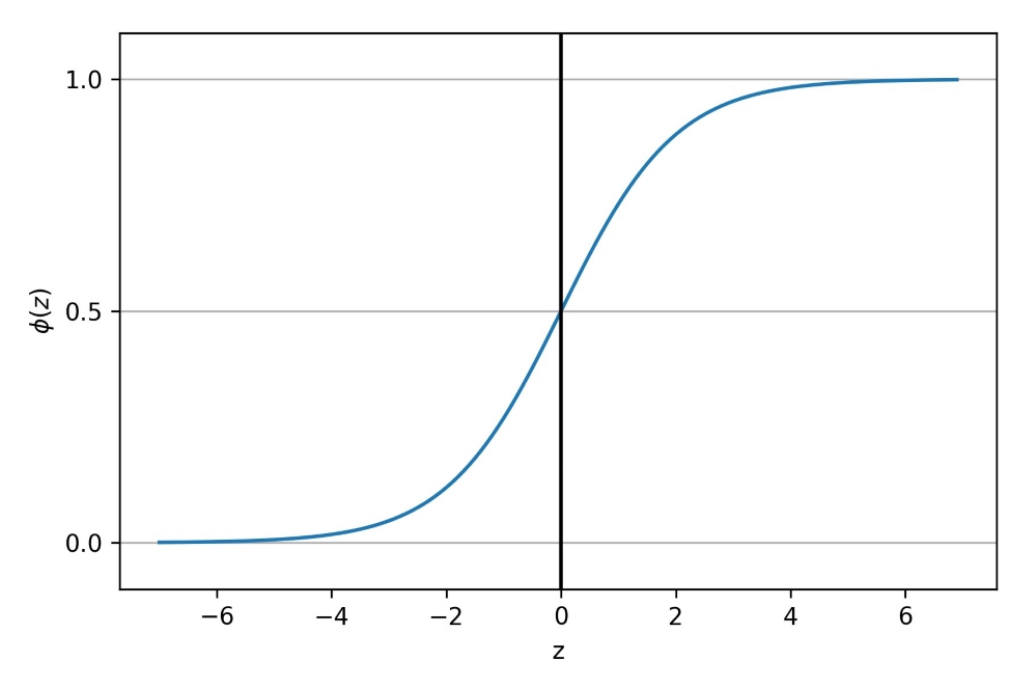
\includegraphics[width=1\linewidth,trim=4 4 4 4,clip]{img/sigmoid.png}
        \caption{Logistic sigmoid function $\phi(z) = \frac{1} {1 + e^{-z}}$ is the inverse form of the logit (log-odds) function.
        It can be used to predict the probability that a certain sample belongs to a particular class.
        The sigmoid function takes real number values as input and transforms them into values in the range [0, 1] with an intercept at $\phi(z) = 0.5$.}
        \label{fig:sigmoid}
    \end{figure}


    Now, we are actually interested in predicting the probability that a certain sample belongs to a particular class, which is the \textbf{inverse form of the logit function}.
    It is also called \textbf{logistic sigmoid function}, sometimes simply abbreviated to sigmoid function due to its characteristic S-shape:

    \begin{equation}
        \label{eq:sigmoid}
        \large{ \phi(z) = \frac{1} {1 + e^{-z}} }
    \end{equation}

    Here z is the net input, the linear combination of weights and sample features:

    \begin{equation}
        \label{eq:net_input}
        z = \vect{w}^T \vect{x} = w_0 x_0 + w_1 x_1 + \dots + w_m x_m
    \end{equation}

    where $w_0$ refers to the bias unit, and is an additional input value that we provide $x_0$, which is set equal to 1.

    On figure~\ref{fig:sigmoid} we can see the general shape of the sigmoid function plotted for some values in the range -7 to 7.

    We can see that $\phi(z)$ approaches 1 if z goes towards infinity ($z \to \infty$) since $e^{-z}$ becomes very small for large values of z.
    Similarly, $\phi(z)$ goes towards 0 for $z \to -\infty$ as a result of an increasingly large denominator.
    Thus, we conclude that this sigmoid function takes real number values as input and transforms them into values in the range [0, 1] with an intercept at $\phi(z) = 0.5$.

    \subsection{Logistic regression compared to Adaline} \label{subsec:lr_ada}

    To build some intuition for the logistic regression model, we can relate it to Adaline, where we used the identity function $\phi(z) = z$ as the activation function.
    In logistic regression, this activation function simply becomes the sigmoid function that was defined in equation~\ref{eq:sigmoid}.
    The difference between Adaline and logistic regression is illustrated in figure~\ref{fig:lr_ada}.

    \begin{figure}[hbt!]
        \centering
        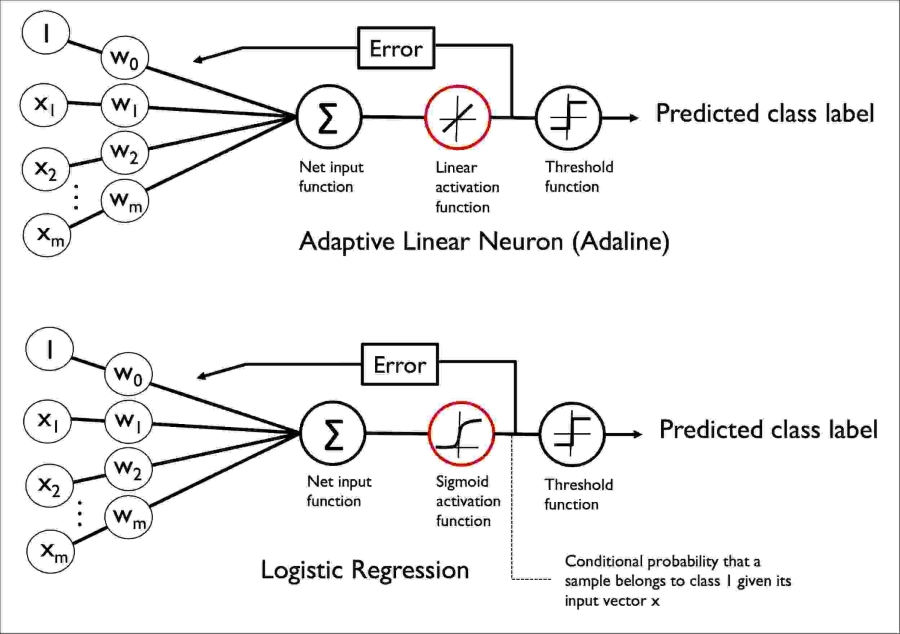
\includegraphics[width=1\linewidth,trim=1 1 1 1,clip]{img/lr_vs_adaline.jpg}
        \caption{Adaline uses the identity function $\phi(z) = z$ as the activation function.
        In logistic regression, this activation function simply becomes the sigmoid function $\phi(z) = \frac{1} {1 + e^{-z}}$ }
        \label{fig:lr_ada}
    \end{figure}

    \subsection{Interpreting the output of the sigmoid function} \label{subsec:lr_sig_interp}

    The output of the sigmoid function in Logistic Regression is interpreted as the probability of a particular sample belonging to class 1 given its features $\vect{x}$ parameterized by the weights $\vect{w}$:

    \begin{equation}
        \label{eq:lr_interp}
        \phi(z) = P( y = 1 | \vect{x}; \vect{w})
    \end{equation}

    For example, if we compute $\phi(z) = 0.8$ for a particular flower sample, it means that the chance that this sample is an Iris-versicolor flower is 80 percent.
    Therefore, the probability that this flower is an Iris-setosa flower can be calculated as $ P( y = 0 | \vect{x}; \vect{w}) = 1 - P( y = 0 | \vect{x}; \vect{w}) = 0.2 $ or 20 percent.
    The predicted probability can then simply be converted into a binary outcome via a threshold function shown in equation~\ref{eq:lr_func_thres}.

    \begin{equation}
        \label{eq:lr_func_thres}
        \hat{y} =
        \begin{cases}
            1 & {\text{if }}\ \phi(z) \geq 0.5, \\
            0 & {\text{otherwise}}
        \end{cases}
    \end{equation}


    If we look at the plot of the sigmoid function presented in figure~\ref{fig:sigmoid}, this is equivalent to the following:

    \begin{equation}
        \hat{y} =
        \begin{cases}
            1 & {\text{if }}\ z \geq 0.0, \\
            0 & {\text{otherwise}}
        \end{cases}
    \end{equation}

    In fact, there are many applications where we are not only interested in the predicted class labels, but where the estimation of the class-membership probability is particularly useful (the output of the sigmoid function prior to applying the threshold function).
    Logistic regression is used in weather forecasting, for example, not only to predict if it will rain on a particular day but also to report the chance of rain.
    Similarly, logistic regression can be used to predict the chance that a patient has a particular disease given certain symptoms, which is why logistic regression enjoys great popularity in the field of medicine.

    \section{Learning the weights of the logistic cost function} \label{sec:lr_weights}

    We saw how we could use the logistic regression model to predict probabilities and class labels;
    now, let us briefly talk about how we fit the parameters of the model, for instance the weights $\vect{w}$.

    \subsection{Continuous cost function Sum-squared-error (SSE)} \label{subsec:sse}

    We defined the sum-squared-error cost function as follows:

    \begin{equation}
        \label{eq:cost_sse}
        J(\boldsymbol{w}) = \sum \limits_i \frac{1} {2} \left( \phi \left( z^{(i)} \right) - y^{(i)} \right) ^2
    \end{equation}

    We minimized this function in order to learn the weights $\vect{w}$ for our Adaline classification model.

    \subsection{Cost function in Logistic Regression \textemdash log-likelihood} \label{subsec:lr_cost}

    To explain how we can derive the cost function for logistic regression, let's first define the \textbf{likelihood L} that we want to maximize when we build a logistic regression model.

    \begin{equation}
        \label{eq:lr_like}
        L(\vect{w}) = P(y|\vect{x};\vect{w}) =
        \prod \limits_{i=1}^n P \left( y^{(i)} | \vect{x}^{(i)}; \vect{w}\right) =
        \prod \limits_{i=1}^{n} \left( \phi \left( z^{(i)} \right) \right)^{y^{(i)}} \left( 1 - \phi \left( z^{(i)} \right) \right)^{1 - y^{(i)}}
    \end{equation}

    In practice, it is easier to maximize the (natural) log of this equation, which is called the \textbf{log-likelihood function}:

    \begin{equation}
        \label{eq:lr_log_like}
        l(\vect{w}) =
        \log L( \vect{w} ) =
        \sum \limits_{i=1}^n \left[ y^{(i)} \log \left( \phi \left( z^{(i)} \right) \right) + \left( 1 - y^{(i)} \right) \log \left( 1 - \phi \left( z^{(i)} \right) \right) \right]
    \end{equation}

    Firstly, applying the log function reduces the potential for numerical underflow, which can occur if the likelihoods are very small.
    Secondly, we can convert the product of factors into a summation of factors, which makes it easier to obtain the derivative of this function via the addition trick, as you may remember from calculus.

    \begin{figure}[hbt!]
        \centering
        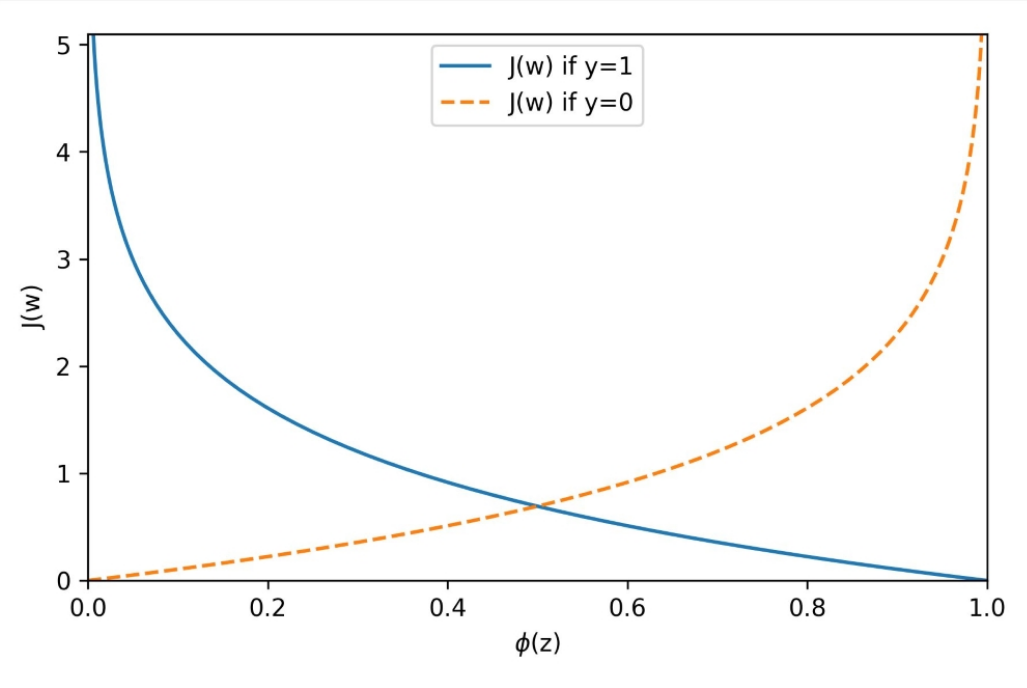
\includegraphics[width=1\linewidth,trim=1 1 1 1,clip]{img/lr_cost.png}
        \caption{Cost of classifying a single-sample instance for different values of $\phi(z)$ (sigmoid activation on the x axis, in the range 0 to 1 and the associated logistic cost on the y-axis).
        If the prediction is wrong, the cost goes towards infinity, this way we penalize wrong predictions with an increasingly larger cost.}
        \label{fig:lr_cost}
    \end{figure}

    \subsection{Intuition for cost function used in Logistic Regression} \label{subsec:lr_cost_intu}

    To get a better grasp of this cost function, let us take a look at the cost that we calculate for one single-sample training instance:

    \begin{equation}
        \label{eq:lr_cost1}
        J( \phi(z), y; \vect{w}) =
        - y \log \left( \phi(z) \right) - (1 - y) \log (1 - \phi(z) )
    \end{equation}

    Looking at the equation~\ref{eq:lr_cost1}, we can see that the first term becomes zero if $y=0$, and the second term becomes zero if $y=1$:

    \begin{equation}
        J( \phi(z), y; \vect{w} ) =
        \begin{cases}
            - \log ( \phi (z) ) & {\text{if }}\ y = 1, \\
            - \log ( 1 - \phi (z) ) & {\text{if }}\ y = 0
        \end{cases}
    \end{equation}

    Figure~\ref{fig:lr_cost} illustrates the cost of classifying a single-sample instance for different values of $\phi(z)$:
    The presented plot shows the sigmoid activation on the x axis, in the range \texttt{0} to \texttt{1} (the inputs to the sigmoid function were z values in the range \texttt{-10} to \texttt{10}) and the associated logistic cost on the y-axis.
    We can see that the cost approaches 0 (continuous line) if we correctly predict that a sample belongs to class 1.
    Similarly, we can see on the y-axis that the cost also approaches 0 if we correctly predict $y=0$ (dashed line).
    However, if the prediction is wrong, the cost goes towards infinity.
    The main point is that we \textbf{penalize wrong predictions with an increasingly larger cost}.

    \subsection{The gradient descent learning algorithm for logistic regression} \label{subsec:lr_gd}

    Using calculus, we can show that the weight update in logistic regression via gradient descent is equal to the equation that we used in Adaline.
    Let's start by calculating the partial derivative of the log-likelihood function with respect to the $j^{th}$ weight:

    \begin{equation}
        \label{eq:dloglike_dw}
        \frac{ \partial } {\pa{w_j} } l(\vect{w}) =
        \left( y \frac{1} {\phi(z)} - (1 - y) \frac{1} {1 - \phi(z)} \right) \frac{ \partial } {\pa{w_j}} \phi(z)
    \end{equation}

    Before we continue, let's also calculate the partial derivative of the sigmoid function:

    \begin{equation}
        \label{eq:dsigmoid}
        \begin{split}
            \large{ \frac{ \partial } { \pa{z} } \phi(z) & =
            \frac{ \partial } { \pa{z}} \frac{1} {1 + e^{-z}} =
            \frac{1} {(1 + e^{-z})^2} e^{-z} = \\
            & = \frac{1} {1 + e^{-z}} \left( 1 - \frac{1} {1 + e^{-z}} \right)} =
            \phi (z) (1 - \phi(z) )
        \end{split}
    \end{equation}

    Now, we can re-substitute $ \frac{ \partial } { \partial z } \phi(z) = \phi (z) (1 - \phi(z) ) $ in equation~\ref{eq:dloglike_dw} to obtain the following:

    \begin{equation}
        \label{eq:dloglike_dw_sol}
        \begin{split}
            \frac{ \partial } {\pa{w_j} } l(\vect{w}) & =
            \left( y \frac{1} {\phi(z)} - (1 - y) \frac{1} {1 - \phi(z)} \right) \frac{ \partial } {\pa{w_j}} \phi(z) = \\
            & = \left( y \frac{1} {\phi(z)} - (1 - y) \frac{1} {1 - \phi(z)} \right) \phi (z) (1 - \phi(z) ) \frac{ \partial } {\pa{w_j}} z = \\
            & = \left( y ( 1 - \phi (z) ) - (1 - y) \phi (z) \right) x_j = (y - \phi(z)) x_j
        \end{split}
    \end{equation}

    Remember that the goal is to find the weights that maximize the log-likelihood so that we perform the update for each weight as follows:

    \begin{equation}
        w_j :=
        w_j + \eta \sum \limits_{i=1}^n \left( y^{(i)} - \phi \left( z^{(i)} \right) \right) x_j
    \end{equation}

    Since we update all weights simultaneously, we can write the general update rule as follows:

    \begin{equation}
        \vect{w} := \vect{w} + \Delta \vect{w}
    \end{equation}

    We define $ \Delta \vect{w} $ as follows:

    \begin{equation}
        \Delta \vect{w} = \eta \nabla l( \vect{w} )
    \end{equation}

    Since maximizing the log-likelihood is equal to minimizing the cost function $J$ that we defined earlier, we can write the gradient descent update rule as follows:

    \begin{equation}
        \Delta w_j =
        - \eta \frac{\pa{J}} {\pa{w_j} } =
        \eta \sum \limits_{i=1}^n \left( y^{(i)} - \phi \left( z^{(i)} \right) \right) x^{(i)}_j
    \end{equation}

    \begin{equation}
        \vect{w} :=
        \vect{w} + \Delta \vect{w}
    \end{equation}

    \begin{equation}
        \Delta \vect{w}
        = - \eta \nabla J( \vect{w} )
    \end{equation}

    This is equal to the gradient descent rule for that we previously used for Adaline.

    \section{An object-oriented Logistic Regression API using NumPy} \label{sec:lr_api}

    \subsection{Converting an Adaline implementation into an algorithm for logistic regression} \label{subsec:ada_to_lr}

    \textit{Raschka and Mirjalili} implement logistic regression simply by substituting the cost function $J$ in their Adaline implementation with the new cost function:

    \begin{equation}
        \label{eq:lr_cost}
        J( \vect{w} ) =
        \sum \limits_{i=1}^n \left[ - y^{(i)} \log \left( \phi \left( z^{(i)} \right) \right) - \left( 1 - y^{(i)} \right) \log \left( 1 - \phi \left( z^{(i)} \right) \right) \right]
    \end{equation}

    This cost function is used to compute the cost of classifying all training samples per epoch.
    Also, linear activation function was swapped with the sigmoid activation and threshold function was changed to return class labels 0 and 1 instead of -1 and 1.
    Making those three changes to the Adaline code results in a working logistic regression implementation.

    \subsection{Iris}
    When we fit a logistic regression model, we have to keep in mind that it only works for binary classification tasks.
    So, let us consider only Iris-setosa and Iris-versicolor flowers (classes 0 and 1) and check that our implementation of logistic regression works:

    \medskip
    \bibliography{lr}
    \bibliographystyle{ieeetr}

\end{document}